\documentclass[norsk,a4paper,12pt]{article}
\usepackage[T1]{fontenc} %for å bruke æøå
\usepackage[utf8]{inputenc}
\usepackage{graphicx} %for å inkludere grafikk
\usepackage{verbatim} %for å inkludere filer med tegn LaTeX ikke liker
\usepackage{amsfonts}
%\usepackage[framed]{mcode} %for å få inn matlabkode
\usepackage{listings}
\usepackage[margin=1.2cm]{caption} % skalere figur text
\usepackage{subfigure}

\bibliographystyle{plain}
\usepackage{parskip}
\usepackage{babel, textcomp, color, amsmath, amssymb, tikz, subfig, float}
\renewcommand{\captionfont}{\sffamily\small} 
\renewcommand{\captionlabelfont}{\bf} 
\fboxsep=0mm % ramme inn bilder


\title{FYS3120 - Midterm Exam}
\author{Kandidate **}
\date{\today}


\begin{document}

\maketitle

%\begin{center}
%Skrive noe smart her? GIT link?
%\end{center}


\newpage


\section*{Abstract}

\section*{Introduction}

\section*{Solution}

\section*{Results}

\section*{Conclusion}


%\subsection*{}

%\begin{figure}[H]
%  \begin{center}
%    \subfigure[N = 10]{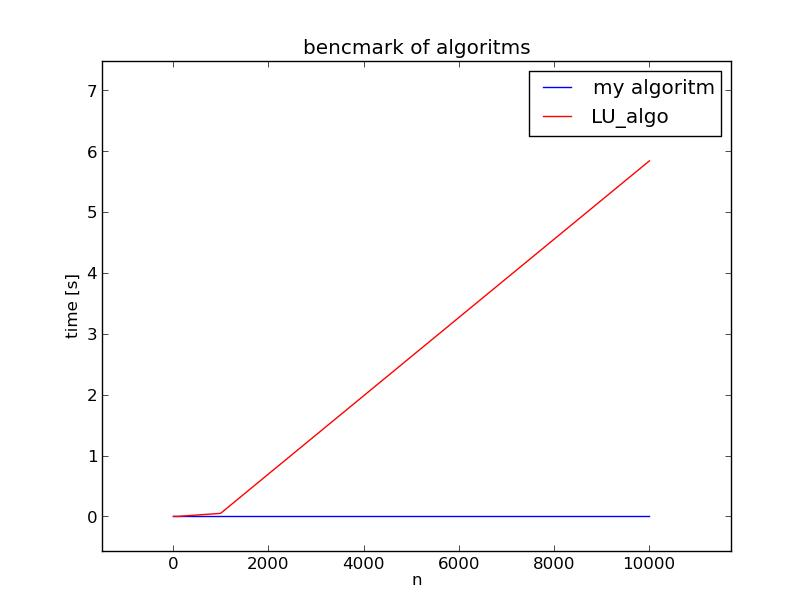
\includegraphics[scale=0.5]{benchmark.jpg}}
%  \end{center}
% \caption{\textit{plot benchmark times for the two different methods of solving}}
%  \label{fig:edge}
%\end{figure}

 
\newpage

\section*{Attachments}

%\textbf{Attachment 1: C++ main program}\newline

%\lstinputlisting[language=C++]{main.cpp}

%\newpage

\end{document}








